%%%%%%%%%%%%%%%%%%%%%%%%%%%%%%%%%%%%%%%%%
% Short Sectioned Assignment LaTeX Template Version 1.0 (5/5/12)
% This template has been downloaded from: http://www.LaTeXTemplates.com
% Original author:  Frits Wenneker (http://www.howtotex.com)
% License: CC BY-NC-SA 3.0 (http://creativecommons.org/licenses/by-nc-sa/3.0/)
%%%%%%%%%%%%%%%%%%%%%%%%%%%%%%%%%%%%%%%%%

%----------------------------------------------------------------------------------------
%	PACKAGES AND OTHER DOCUMENT CONFIGURATIONS
%----------------------------------------------------------------------------------------

\documentclass[paper=a4, fontsize=11pt]{scrartcl} % A4 paper and 11pt font size

% ---- Entrada y salida de texto -----

\usepackage[T1]{fontenc} % Use 8-bit encoding that has 256 glyphs
\usepackage[utf8]{inputenc}
%\usepackage{fourier} % Use the Adobe Utopia font for the document - comment this line to return to the LaTeX default

% ---- Idioma --------

\usepackage[spanish, es-tabla]{babel} % Selecciona el español para palabras introducidas automáticamente, p.ej. "septiembre" en la fecha y especifica que se use la palabra Tabla en vez de Cuadro

% ---- Otros paquetes ----

\usepackage{url} % ,href} %para incluir URLs e hipervínculos dentro del texto (aunque hay que instalar href)
\usepackage{amsmath,amsfonts,amsthm} % Math packages
%\usepackage{graphics,graphicx, floatrow} %para incluir imágenes y notas en las imágenes
\usepackage{graphics,graphicx, float} %para incluir imágenes y colocarlas

% Para hacer tablas comlejas
%\usepackage{multirow}
%\usepackage{threeparttable}

%\usepackage{sectsty} % Allows customizing section commands
%\allsectionsfont{\centering \normalfont\scshape} % Make all sections centered, the default font and small caps

\usepackage{fancyhdr} % Custom headers and footers
\pagestyle{fancyplain} % Makes all pages in the document conform to the custom headers and footers
\fancyhead{} % No page header - if you want one, create it in the same way as the footers below
\fancyfoot[L]{} % Empty left footer
\fancyfoot[C]{} % Empty center footer
\fancyfoot[R]{\thepage} % Page numbering for right footer
\renewcommand{\headrulewidth}{0pt} % Remove header underlines
\renewcommand{\footrulewidth}{0pt} % Remove footer underlines
\setlength{\headheight}{13.6pt} % Customize the height of the header

\numberwithin{equation}{section} % Number equations within sections (i.e. 1.1, 1.2, 2.1, 2.2 instead of 1, 2, 3, 4)
\numberwithin{figure}{section} % Number figures within sections (i.e. 1.1, 1.2, 2.1, 2.2 instead of 1, 2, 3, 4)
\numberwithin{table}{section} % Number tables within sections (i.e. 1.1, 1.2, 2.1, 2.2 instead of 1, 2, 3, 4)

\setlength\parindent{0pt} % Removes all indentation from paragraphs - comment this line for an assignment with lots of text

\newcommand{\horrule}[1]{\rule{\linewidth}{#1}} % Create horizontal rule command with 1 argument of height

\graphicspath{ {./images/} }
\usepackage{subcaption}
\usepackage{hyperref}
\usepackage{soul}

\setlength{\parskip}{10px}


%----------------------------------------------------------------------------------------
%	TÍTULO Y DATOS DEL ALUMNO
%----------------------------------------------------------------------------------------

\title{	
\normalfont \normalsize 
\textsc{\textbf{Aprendizaje Automático (2019)} \\ Doble Grado en Ingeniería Informática y Matemáticas \\ Universidad de Granada} \\ [25pt] % Your university, school and/or department name(s)
\horrule{0.5pt} \\[0.4cm] % Thin top horizontal rule
\huge Proyecto Final \\ % The assignment title
\horrule{2pt} \\[0.5cm] % Thick bottom horizontal rule
}

\author{Ignacio Aguilera Martos, Luis Balderas Ruiz \\ \texttt{nacheteam@correo.ugr.es, luisbalderas@correo.ugr.es}} 
 % Nombre y apellidos 


\date{\normalsize\today} % Incluye la fecha actual

%----------------------------------------------------------------------------------------
% DOCUMENTO
%----------------------------------------------------------------------------------------

\begin{document}

\maketitle % Muestra el Título

\newpage %inserta un salto de página

\tableofcontents % para generar el índice de contenidos

\listoffigures

\listoftables

\newpage


%----------------------------------------------------------------------------------------
%	Introducción
%----------------------------------------------------------------------------------------

\section{APS Failure Scania Trucks Classification}

\subsection{Introducción}

Nos encontramos ante un problema de clasificación binaria (clase positiva y negativa) en la que la clase positiva consiste en el fallo o mal funcionamiento de un componente específico del sistema APS para la compañía de camiones Scania. Por su parte, la clase negativa está formada por camiones con fallos en componentes que no están relacionado con el sistema APS. En lo que se refiere al dataset en sí, el conjunto de entrenamiento está formado por 60000 instancias y 171 características. El test tiene 16000 muestras. Sabemos que los nombres de los atributos han sido anonimizados por motivos de privacidad. En el presente documento explicamos con detalle cada uno de los pasos que hemos seguido en el estudio y diseño de un sistema inteligente para la clasificación con varios modelos, a saber, un modelo lineal (SGD), una Máquina de Soporte de Vectores, un modelo basado en Boosting (AdaBoost, concretamente) y Random Forest. Previo uso de los modelos, hemos hecho un profundo estudio de los datos que nos han llevado a modificarlos y tratarlos para mejorar los resultados, entre lo que destaca el tratamiento de valores perdidos con la imputación de la mediana, eliminación de estancias poco relevantes, oversampling con SMOTE para compensar el gran desbalanceo y análisis factorial para reducir la dimensionalidad en las características. 

\section{Preprocesamiento}

\subsection{Análisis explotario y valores perdidos}

Nos encontramos ante un problema que tiene una gran cantidad de datos. En principio, este hecho es una ventaja, dado que la capacidad de generalización aumenta enormemente. Sin embargo, uno de los grandes retos ha sido, por un lado, el gran desbalanceo entre las clases y, por otro, la gran cantidad de valores perdidos e inconsistencias en los datos. Nos ocupamos de esto segundo en primer lugar. El análisis exploratorio de los datos nos hizo llegar a la conclusión de que, de entre las pocas instancias que forman parte de la clase positiva (esto es, con un fallo en el sistema APS), los valores de las variables estaban extraviados o, si no era así, más parecían outliers que otra cosa. En seguida nos dimos cuenta de que, desde un punto de vista físico tiene sentido, dado que la avería en un componente puede hacer que el comportamiento en los demás sea errático y, como consecuencia, puede generar observaciones de lo más variopintas. No obstante, nos dedicamos a eliminar los valores perdidos y le dimos validez total a los datos de los que disponemos. 

En primer, vimos que había características que tenían más de un 70\% de sus valores como NA. Decidimos eliminarlas, ya que iban a entorpecer enormemente el trabajo de los modelos (en alguno de ellos, incluso son incompatibles). Eliminamos por tanto las características 2,75,76,77,78,79 y 113, por lo que pasamos de 171 a 164. En lo que se refiere a instancias, observamos que gran cantidad de ellas también estaban pobladas de valores perdidos. Teniendo en cuenta el gran desbalanceo de las clases, eliminamos aquellas instancias con etiqueta negativa que tuvieran más de un 15\% de sus entradas como NA, de forma que pasamos de 60000 instancias a 55964. 

A partir de ahí, nuestro conjunto de datos es más tratable. Sin embargo, aunque más dispersos, aún hay muchos valores perdidos con los que los modelos no pueden lidiar. Para solucionarlo, consultando la bibliografía, utilizamos dos tipos de imputación de valores perdidos: imputación de la mediana y de la media. La mediana nos ha dado mejores resultados en general, por lo que continuamos nuestro desarrollo con la mediana. 

\subsubsection{Desbalanceo de clases}

Sin duda alguna, uno de los grandes problemas a los que nos enfrentamos cuando tratamos este conjunto de datos es el gran desbalanceo entre las clases. Hicimos una primera visualización de los datos observando el desbalanceo pero, a su vez, leve solapamiento (lo que a priori es una ventaja).

\begin{figure}[H] %con el [H] le obligamos a situar aquí la figura
		\centering
		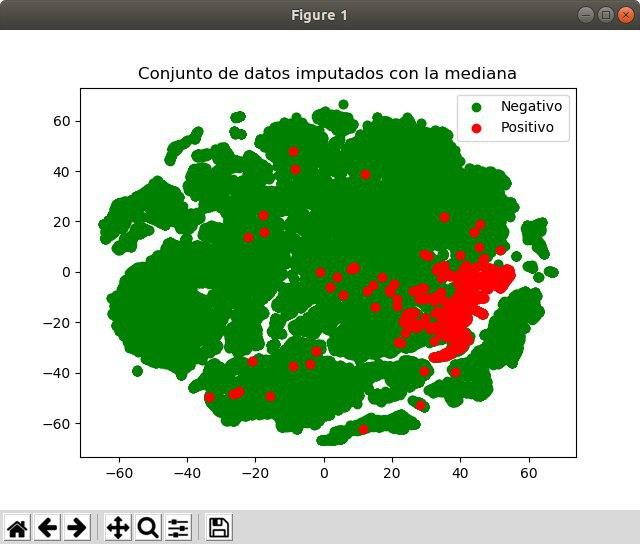
\includegraphics[scale=0.6]{pre-smote.jpg}  %el parámetro scale permite agrandar o achicar la imagen. En el nombre de archivo puede especificar directorios
		\caption{Representación de las instancias tras la imputación de VP con la mediana} 
	\label{fig:sep-clases}
\end{figure}

Sin embargo, a pesar de la separación de las clases éramos incapaces de generar buenos resultados con los modelos y los clasificadores siempre etiquetaban las instancias de test como pertenecientes a la clase negativa. Esto daba lugar a un buen accuracy, pero las demás medidas que tenemos en cuenta, como son recall o f1-score eran nefastas.

\begin{figure}[H] %con el [H] le obligamos a situar aquí la figura
	\centering
	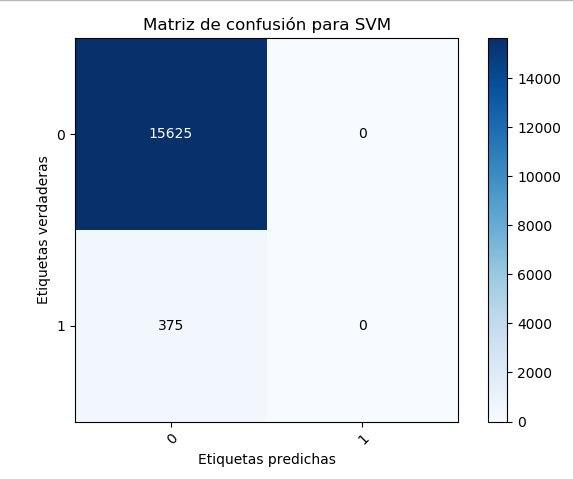
\includegraphics[scale=0.6]{conf1.jpg}  %el parámetro scale permite agrandar o achicar la imagen. En el nombre de archivo puede especificar directorios
	\caption{Matriz de confusión generada por SVM /RF/SGD/Red Neuronal hasta el momento} 
	\label{fig:conf1}
\end{figure}

Por tanto, a pesar de la buena disposición de los datos, no se obtenían buenos resultados. A la vista de los mismos, nos decantamos por utilizar técnicas de oversampling para equilibrar el número de instancias de cada clase. En particular, elegimos SMOTE (\cite{smote}) como herramienta. Tras su aplicación, contamos finalmente con 109928 instancias de cada clase, apareciendo la siguiente disposición de datos:

\begin{figure}[H] %con el [H] le obligamos a situar aquí la figura
	\centering
	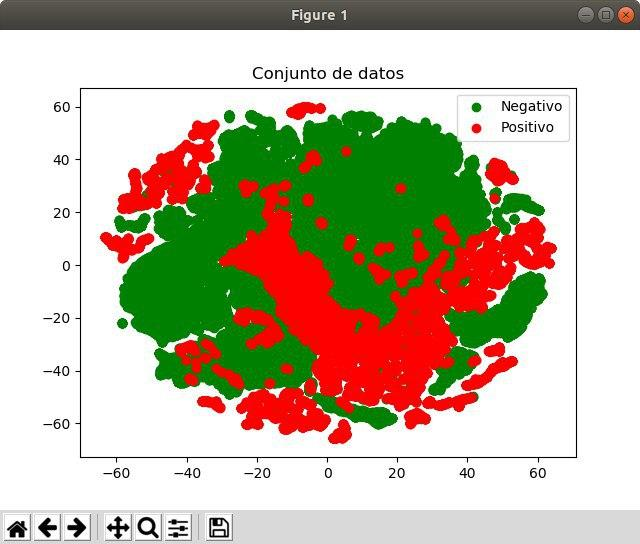
\includegraphics[scale=0.55]{tras-smote.jpg}  %el parámetro scale permite agrandar o achicar la imagen. En el nombre de archivo puede especificar directorios
	\caption{Disposición del dataset tras SMOTE} 
	\label{fig:post-smote}
\end{figure}

Como se puede apreciar, hemos perdido la localidad de las clases, aunque, como se verá, va a ser muy positivo.

\subsubsection{Selección de características}

Tras la eliminación de características por poseer demasiados valores perdidos, poseemos 164. No nos parece un número adecuado para utilizar PCA (más recomendado para cuando hay muchas más variables, ya que el sacrificio de la interpretabilidad es menos costoso) así que nos decantamos por otras técnicas de estadística multivariante, como es análisis factorial (\cite{ms},\cite{amsa},\cite{fa1}, \cite{fa2}). Análisis factorial sí nos ayuda a darle interpretabilidad al modelo y a encontrar qué características son las más determinantes. Reducimos así de 164 a 151. Sin embargo, los resultados en los modelos nos harán comprobar que, a pesar de mejorar el accuracy, se empeora la clasificación de las instancias de la clase positiva, como se puede ver en la siguiente comparación entre matrices de confunsión para Random Forest:

\begin{table}[H]
	\centering
	\begin{tabular}{|c|c|c|}
		\hline
		Verd \textbackslash Pred & 0     & 1    \\ \hline
		0                        & 56160 & 2840 \\ \hline
		1                        & 77    & 923  \\ \hline
	\end{tabular}
	\caption{Matriz de confusión sin FA}
\end{table}

\begin{table}[H]
	\centering
	\begin{tabular}{|c|c|c|}
		\hline
		Verd \textbackslash Pred & 0     & 1    \\ \hline
		0                        & 57077 & 1923 \\ \hline
		1                        & 113   & 887  \\ \hline
	\end{tabular}
	\caption{Matriz de confusión con FA}
\end{table}

Por tanto, como nuestro objetivo es maximizar todas las medidas, especialmente recall (la clase minoritaria sigue siendo, de forma natural, la clase positiva), optamos por no aplicar de forma definitiva análisis factorial. Después de explorar estas dos técnicas, llegamos a la conclusión de que el tamaño del dataset hace que el número de características no sea muy elevado, por lo que acabamos por no seleccionar ningún subconjunto de ellas.

\subsubsection{Normalización}

En el análisis exploratorio observamos que el rango de las variables es absolutamente dispar. Todos los clasificadores basados en instancias (que incorporan la distancia) necesitan de un rango de variables equivalente para poder dar el peso adecuada a cada una. Por eso, realizamos una normalización estándar a los datos.

\section{Modelos y clasificación}

\subsection{Error de generalización y dimensión de VC}

	
Pueden calcularse dos cotas (\cite{lfd}). Trato primera la de $E_{in}$. 
Sea $h \in H$, fija, $f(x)$ la función objetivo (desconocida), $D$ el conjunto de entrenamiento de tamaño N. Podemos escribir la desigualdad de Hoeffding como sigue:

$$P(D: |E_{out}(h)-E_{in}(h)|> \epsilon) \leq 2 e^{-2\epsilon^2N} \hspace{0.5cm} \forall \epsilon > 0$$

Llamando $\delta = 2e^{-2\epsilon^2 N}$, tenemos

$$P(D: |E_{out}(h)-E_{in}(h)|> \epsilon) \leq \delta \Rightarrow P(D: |E_{out}(h)-E_{in}(h)| < \epsilon) \geq 1 - \delta$$

Podemos escribir, por tanto, la siguiente desigualdad:

$$E_{out}(h) \leq E_{in}(h) + \sqrt{\frac{1}{2N} \log \frac{2}{\delta}}$$
con probabilidad al menos $1-\delta$ en $D$.

Considerando una clase de funciones finita, la expresión se convierte en 
$$E_{out}(h) \leq E_{in}(h) + \sqrt{\frac{1}{2N} \log \frac{2|H|}{\delta}}$$

Sin embargo, el tamaño de la clase de funciones ahora entra en juego y puede hacer menos útil la cota. Para poder garantizar una buena cota, surge la teoría de la generalización y la Dimensión de Vapnik-Chervonenkis (VC). La cota a utilizar es la siguiente:

$$E_{out}(h) \leq E_{in}(h) + \sqrt{\frac{8}{N} \log \frac{4((2N)^{d {VC}}+1)}{\delta}}$$


Para el caso de $E_{test}$, cuando afirmamos que $E_{test}$ es un estimador de $E_{out}$, estamos afirmando que $E_{test}$ generaliza muy bien $E_{out}$. En el caso anterior, intentábamos buscar la función que minimizaba $E_{in}$. Ahora, sin embargo, ya tenemos una función fija y queremos simplemente estimar el error. Por tanto, la desigualdad de Hoeffding con una hipótesis es suficiente para el caso de conjunto de test. 

$$E_{out}(h) \leq E_{test}(h) + \sqrt{\frac{1}{2N} \log \frac{2}{\delta}}$$

En cada caso, utilizaremos la que más convenga. En los modelos en los que la dimensión de VC sea excesivamente elevada (debido a la complejidad, como las redes y los basados en árboles, incluso infinita) utilizaremos exclusivamente la que involucra a $E_{test}$.

\subsection{Gradiente descendente estocástico}


El primer modelo que utilizamos es Gradiente Descendente Estocástico. Establecemos un número máximo de iteraciones de 10000 y una tolerancia de $1^{-6}$. Se produce la convergencia tras 46 épocas con los siguientes resultados:

\begin{table}[H]
	\centering
	\begin{tabular}{|c|c|}
		\hline
		Score     & 0.97105    \\ \hline
		Precision & 0.9883861  \\ \hline
		Recall    & 0.97105    \\ \hline
		F1-Score  & 0.97734082 \\ \hline
	\end{tabular}
	\caption{Resumen de las medidas obtenidas con SGD}
\end{table}

Además, obtenemos la siguiente matriz de confusión:

\begin{figure}[H] %con el [H] le obligamos a situar aquí la figura
	\centering
	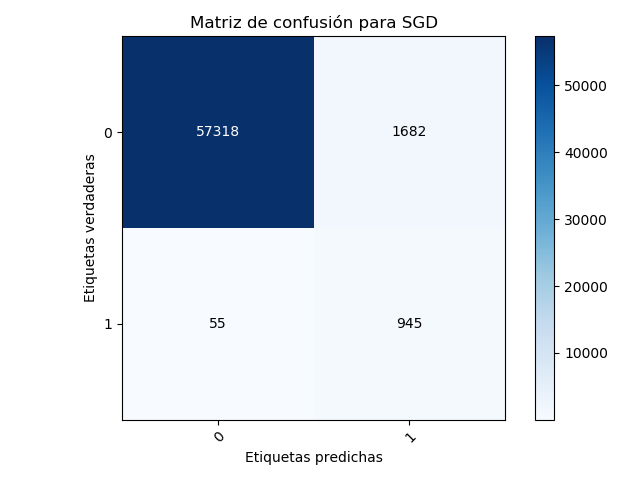
\includegraphics[scale=0.6]{SGDConf.png}  %el parámetro scale permite agrandar o achicar la imagen. En el nombre de archivo puede especificar directorios
	\caption{Matriz de confusión para SGD} 
	\label{fig:sgd-conf}
\end{figure}

y la siguiente curva ROC:

\begin{figure}[H] %con el [H] le obligamos a situar aquí la figura
	\centering
	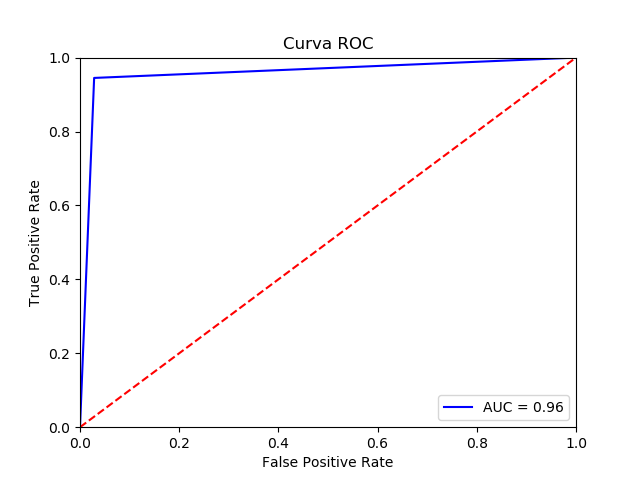
\includegraphics[scale=0.6]{ROC-SGD.png}  %el parámetro scale permite agrandar o achicar la imagen. En el nombre de archivo puede especificar directorios
	\caption{Curva ROC para SGD} 
	\label{fig:roc-sgd}
\end{figure}

Como se puede ver, los resultados son altamente satisfactorios. Además, con un problema que posee un volumen de datos tan grande, el tiempo de computación es un factor a tener en cuenta, y, en efecto, SGD apenas tarda un minuto en concluir. 

Como se trata de un modelo lineal, dimensión de VC = 3, por lo que la cota de generalización a través de $E_{in} = 0.02063704531572863$ vale:
$$E_{out} \leq 0.08529664599521261$$

Con respecto a la segunda forma de calcularlo (con $E_{test}=0.02895000000000003$),

$$E_{out} \leq 0.033845879766038436$$

Nos quedamos con la segunda por ser más pequeña.
\subsubsection{AdaBoost}

El segundo modelo empleado es la implementación de Boosting conocida como AdaBoost con un parámetro de estimadores de 100. 

\begin{table}[H]
	\centering
	\begin{tabular}{|c|c|}
		\hline
		Score     & 0.9694   \\ \hline
		Precision & 0.98717  \\ \hline
		Recall    & 0.9694   \\ \hline
		F1-Score  & 0.976038 \\ \hline
	\end{tabular}
	\caption{Resumen de las medidas obtenidas con AdaBoost}
\end{table}

Como podemos ver los resultados obtenidos son satisfactorios, vamos a ver ahora la matriz de confusión para tener una idea mejor y más completa del resultado.

\begin{figure}[H] %con el [H] le obligamos a situar aquí la figura
	\centering
	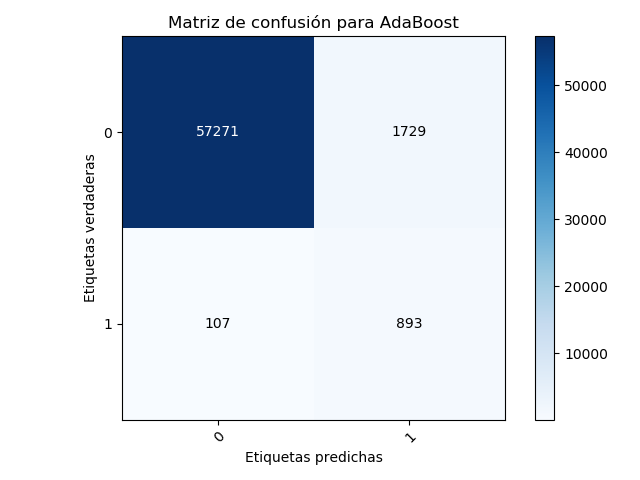
\includegraphics[scale=0.6]{AdaBoostConf.png}  %el parámetro scale permite agrandar o achicar la imagen. En el nombre de archivo puede especificar directorios
	\caption{Matriz de confusión para AdaBoost} 
	\label{fig:conf-adaboost}
\end{figure}

Analizando ahora el resultado podemos ver que la variable más determinante, que en nuestro caso es acertar las etiquetas 1 (los fallos en frenos) es menor que en el caso de SGD, es decir en SGD obtenemos una mayor tasa de acierto en los verdaderos positivos de la clase 1 por lo que de momento nos interesa más dicho modelo que Boosting.

Podemos visualizar asimismo la curva ROC.

\begin{figure}[H] %con el [H] le obligamos a situar aquí la figura
	\centering
	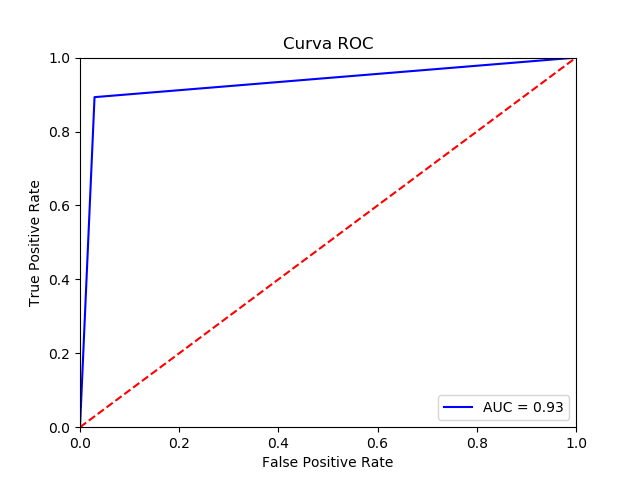
\includegraphics[scale=0.6]{ROC-AB.png}  %el parámetro scale permite agrandar o achicar la imagen. En el nombre de archivo puede especificar directorios
	\caption{Curva ROC para AdaBoost} 
	\label{fig:roc-ab}
\end{figure}

Respecto de la cota de generalización, tiendo un $E_{in}= 0.013333506608273038$ y un $E_{test} = 0.03059999999999996$, obtenemos que

$$E_{out} \leq 0.035495879766038366$$


\subsubsection{Red Neuronal (Perceptrón multicapa)}

El tercer modelo empleado ha sido una Red Neuronal, en concreto un Perceptrón Multicapa. Los parámetros empleados en el modelo han sido 3 capas con 100 estimadores simples por capa, con un número máximo de iteraciones de 10000. La convergencia del modelo se produce mucho antes de estas iteraciones máximas, en concreto en la iteración 63. Los resultados han sido:

\begin{table}[H]
	\centering
	\begin{tabular}{|c|c|}
		\hline
		Score     & 0.98575   \\ \hline
		Precision & 0.992269  \\ \hline
		Recall    & 0.98575   \\ \hline
		F1-Score  & 0.98782 \\ \hline
	\end{tabular}
	\caption{Resumen de las medidas obtenidas con Perceptrón Multicapa}
\end{table}

Los resultados generales como podemos ver parecen tremendamente prometedores, vamos a ver la matriz de confusión:

\begin{figure}[H] %con el [H] le obligamos a situar aquí la figura
	\centering
	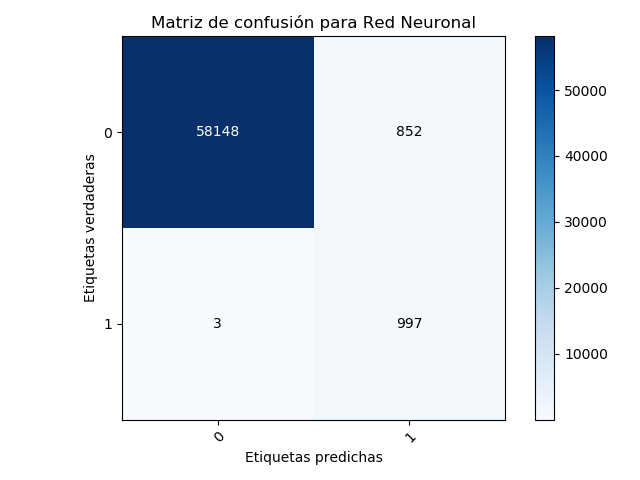
\includegraphics[scale=0.6]{CONF-NEURONAL.png}  %el parámetro scale permite agrandar o achicar la imagen. En el nombre de archivo puede especificar directorios
	\caption{Matriz de confusión para Perceptrón Multicapa} 
	\label{fig:conf-pmc}
\end{figure}

Como podemos ver en este caso se producen 997 aciertos y sólo 3 fallos con lo que hemos conseguido superar incluso el resultado obtenido por Gradiente Descendente Estocástico con el modelo de perceptrón multicapa.

Veamos la curva ROC:

\begin{figure}[H] %con el [H] le obligamos a situar aquí la figura
	\centering
	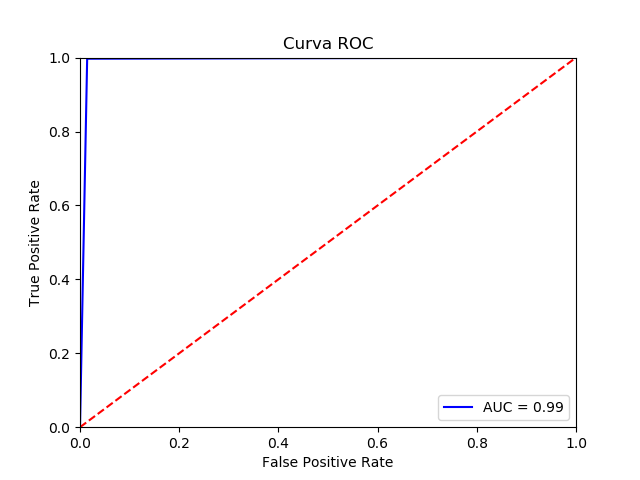
\includegraphics[scale=0.6]{ROC-NEURONAL.png}  %el parámetro scale permite agrandar o achicar la imagen. En el nombre de archivo puede especificar directorios
	\caption{Curva ROC para Perceptrón Multicapa} 
	\label{fig:roc-pmc}
\end{figure}

Respecto de la cota de generalización, tiendo un $E_{in}=0.0010006627766442344 $ y un $E_{test} =0.012399999999999967 $, obtenemos que

$$E_{out} \leq 0.01729587976603837$$


\subsubsection{Random Forest}

El cuarto modelo empleado ha sido un Random Forest. Los parámetros del modelo han sido obtenidos a través de un GridSearch para obtener el mejor número de estimadores o clasificadores simples. En nuestro caso el mejor valor obtenido es con 189 estimadores. Los resultados han sido:

\begin{table}[H]
	\centering
	\begin{tabular}{|c|c|}
		\hline
		Score     & 0.9864   \\ \hline
		Precision & 0.9925  \\ \hline
		Recall    & 0.9864   \\ \hline
		F1-Score  & 0.9883 \\ \hline
	\end{tabular}
	\caption{Resumen de las medidas obtenidas con Random Forest}
\end{table}

Los resultados generales como podemos ver parecen tremendamente prometedores al igual que nos ha ocurrido con la red neuronal, vamos a ver la matriz de confusión:

\begin{figure}[H] %con el [H] le obligamos a situar aquí la figura
	\centering
	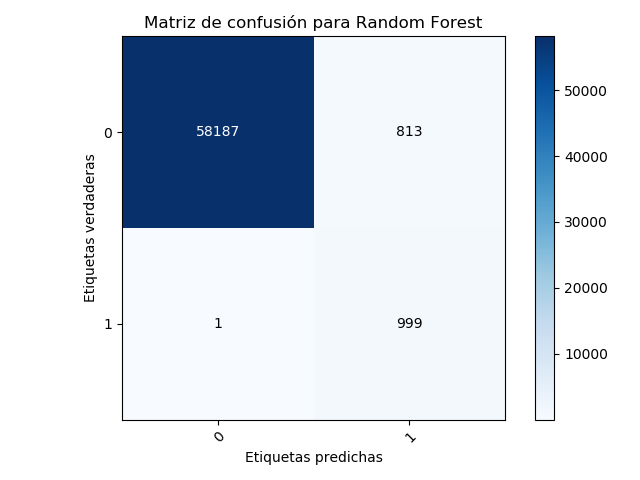
\includegraphics[scale=0.6]{RandomForestConf.png}  %el parámetro scale permite agrandar o achicar la imagen. En el nombre de archivo puede especificar directorios
	\caption{Matriz de confusión para Random Forest} 
	\label{fig:conf-rf}
\end{figure}

Como podemos ver en este caso se producen 999 aciertos y sólo 1 fallos con lo que hemos conseguido superar tanto el resultado obtenido por Gradiente Descendente Estocástico como el modelo de perceptrón multicapa con lo que Random Forest es actualmente el modelo que mejores resultados ha obtenido.

Veamos la curva ROC:

\begin{figure}[H] %con el [H] le obligamos a situar aquí la figura
	\centering
	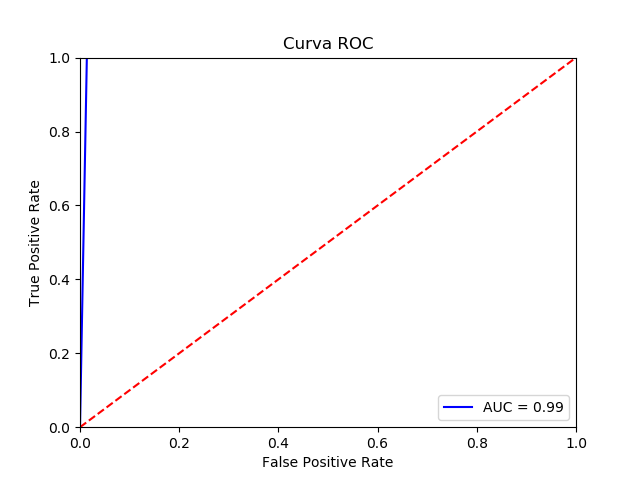
\includegraphics[scale=0.6]{ROC-RF.png}  %el parámetro scale permite agrandar o achicar la imagen. En el nombre de archivo puede especificar directorios
	\caption{Curva ROC para Random Forest} 
	\label{fig:roc-rf}
\end{figure}

En cuanto al error de generalización, dado que $E_in=0, E_{test} = 0.013566666666666616,$ obtenemos la siguiente cota:

$$E_{out} \leq 0.018462546432705017$$

\subsubsection{SVM}

El último modelo empleado ha sido SVM. Los parámetros del modelo han sido obtenidos a través de un GridSearch para obtener los mejores valores de gamma y C tal y como se indica en el PDF. En nuestro caso el mejor valor obtenido de gamma ha sido 0.01 y C 0.95 con el kernel RBF. Los resultados han sido:

\begin{table}[H]
	\centering
	\begin{tabular}{|c|c|}
		\hline
		Score     & 0.97665   \\ \hline
		Precision & 0.98972  \\ \hline
		Recall    & 0.97665   \\ \hline
		F1-Score  & 0.98120 \\ \hline
	\end{tabular}
	\caption{Resumen de las medidas obtenidas con SVM}
\end{table}

Los resultados generales como podemos ver no son tan buenos a priori como en la red neuronal y random forest, aún así vamos a ver la matriz de confusión:

\begin{figure}[H] %con el [H] le obligamos a situar aquí la figura
	\centering
	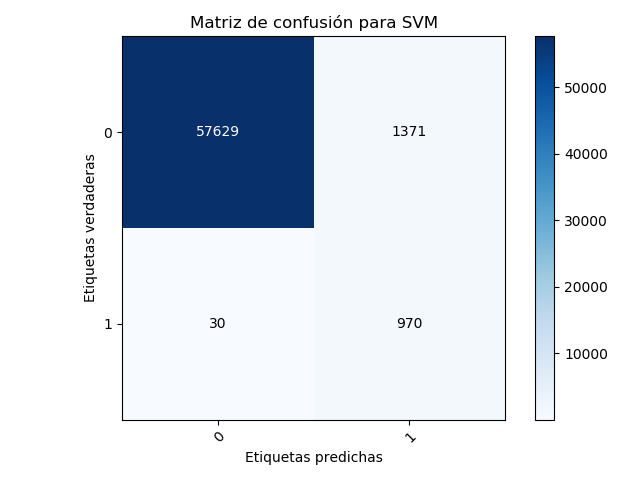
\includegraphics[scale=0.6]{SVM-CONF.png}  %el parámetro scale permite agrandar o achicar la imagen. En el nombre de archivo puede especificar directorios
	\caption{Matriz de confusión para SVM} 
	\label{fig:conf-svm}
\end{figure}

Como podemos ver en este caso se producen 970 aciertos y 30 fallos con lo que este modelo ha conseguido funcionar mejor que SGD y AdaBoost pero no que Random Forest ni Perceptrón multicapa.

Veamos la curva ROC:

\begin{figure}[H] %con el [H] le obligamos a situar aquí la figura
	\centering
	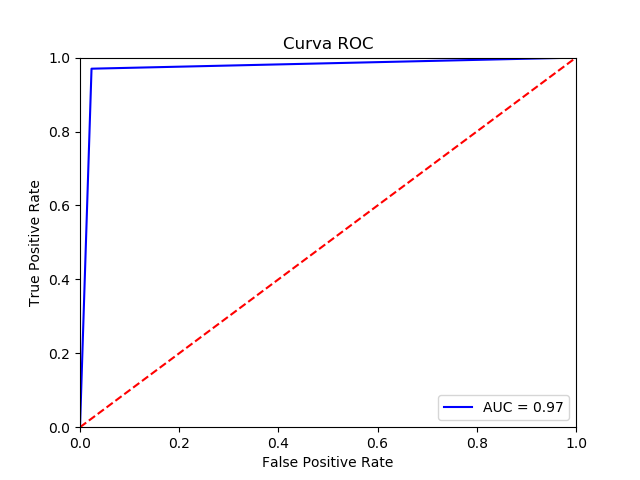
\includegraphics[scale=0.6]{SVM-ROC.png}  %el parámetro scale permite agrandar o achicar la imagen. En el nombre de archivo puede especificar directorios
	\caption{Curva ROC para SVM} 
	\label{fig:roc-svm}
\end{figure}

Respecto de la cota de generalización, tiendo un $E_{in}= 0.011306189814032641$ y un $E_{test} = 0.023349999999999982$, obtenemos que

$$E_{out} \leq 0.028245879766038384$$

\newpage
\section{Bibliografía}

%------------------------------------------------

\bibliography{citas} %archivo citas.bib que contiene las entradas 
\bibliographystyle{plain} % hay varias formas de citar

\end{document}
